\chapter{Úvod}\label{chap:uvod}
\addcontentsline{toc}{chapter}{Úvod}

Spolu s harmonií a rytmem představuje melodie základní stavební kámen většiny existující hudby. V průběhu vývoje od folklórních zpěvů přes orchestrální skladby po soudobou elektroniku si melodie téměř vždy zachovávala své dominantní postavení nositele esence jednotlivých písní. Melodie je to hlavní, co si člověk po poslechu skladby odnáší a nejsnadněji vybaví, a její důležitost je zejména v našem kulturním kontextu natolik jednoznačná, že se hudba, která ji postrádá, zřídkakdy dostává do širokého povědomí.

\begin{figure}[h]\centering
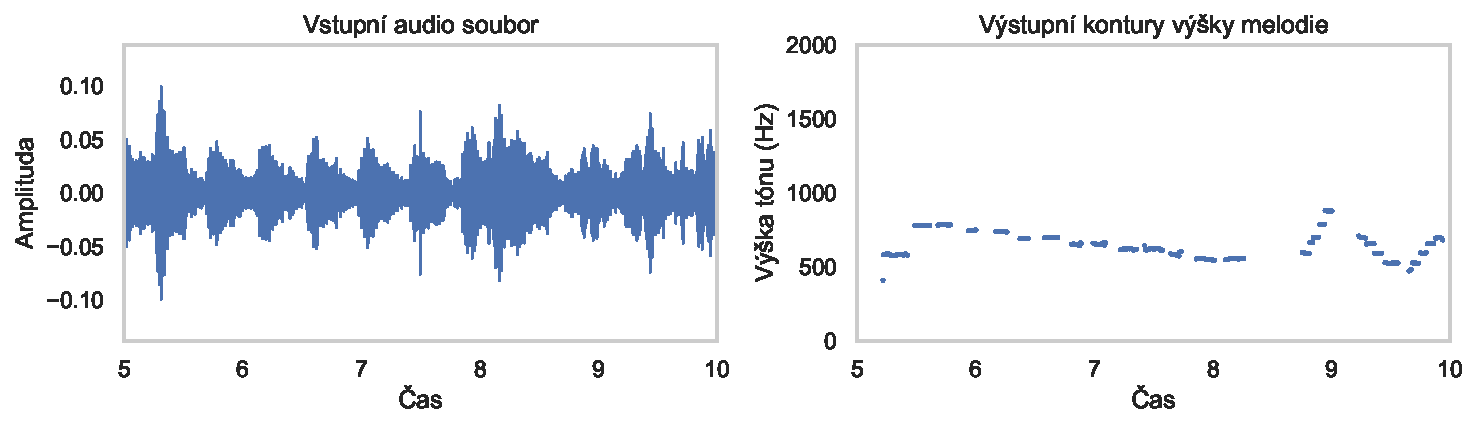
\includegraphics[width=\textwidth,height=\textheight,keepaspectratio]{../img/input_output}
\caption{Příklad vstupu a výstupu metody pro extrakci melodie. \textcolor{red}{přidat zvukový přílkad do přílohy}}
\label{obr:input_output}
\end{figure}

Tato práce se zabývá metodami odhadu fundamentální frekvence melodie ze zvukové nahrávky. Jinými slovy je naším cílem získat v každém bodě vstupní skladby informaci o tom, zda melodie v daném okamžiku zní a její případnou výšku. Jde o jednu z nejdůležitějších a zároveň nejtěžších úloh z oboru \textit{Music Information Retrieval} (MIR), jejíž rozsah využití v této doméně pokrývá významnou část aktivně řešených, otevřených problémů. 

Spolehlivý přepis melodie by usnadnil vyhledávání v hudebních datech, ať už na základě notového zápisu (\textit{Symbolic Melodic Similarity}), pomocí nekvalitní nahrávky z rádia (\textit{Audio Fingerprinting}), pomocí broukání (\textit{Query by Singing/Humming}) nebo dokonce pomocí coveru hledané písně (\textit{Audio Cover Song Identification}). Mimo vyhledávání by byl algoritmus užitečný pro další zpracování zvukového signálu, ať už pro manipulaci a úpravu melodického hlasu (například software Melodyne), nebo naopak jeho odstranění a vytvoření karaoke doprovodu (\textit{Informed Source Separation}). V neposlední řadě by extrakce melodie pomohla při kategorizaci hudebních dat, například podle žánru (\textit{Genre Classification}) nebo podle zpěváka (\textit{Singer Characterization}). A konečně široké spektrum využití by nalezla i v muzikologii (případně etnomuzikologii) pro kvantitativní i kvalitativní studii hudebních motivů a postupů (V jazzu například \cite{Pfleiderer}).

Extrakce melodie však nemusí sloužit pouze jako mezikrok pro řešení jiné úlohy, užitečný je i samotný výstup algoritmu, znázorněný na obrázku \ref{obr:input_output}. Motivačním příkladem použití může být pomoc při transkripci. Představíme-li si začínajícího hráče na saxofon, který si chce do not přepsat své oblíbené jazzové sólo, výstup algoritmu mu dá užitečnou informaci o tom, jaký tón zní v jakou chvíli. Z této reprezentace už pak hráči zbývá nalezené tóny projít a zapsat je do notové osnovy.

\section{Analýza hudebního signálu}

Proč je ale extrakce melodie otevřený problém? Příbuzná úloha, která spočívá v přepisu nahrávky jednoho izolovaného nástroje, je v podstatě vyřešena \citep{Mauch2014a}, proč se tato úloha po přidání hudebního doprovodu stává výrazně obtížnější? Pro vysvětlení zásadního problému, který se s přepisem nahrávky pojí, musíme nejdříve přiblížit vůbec povahu zvuku a možnosti jeho zkoumání.

Naše zkušenost se zvukem probíhá primárně skrze sluch. Teprve na hlasitém koncertu však člověk pocítí, že zvuk je ve své fyzikální podstatě změna tlaku vzduchu, putující od zdroje k posluchači. Díky sluchu z těchto vibrací dokážeme oddělit jednotlivé zdroje a identifikovat v nich i velmi jemné rozdíly. Ačkoli jde o subjektivní vjemy, zvuky lze částečně rozřadit podle toho, jak snadno v nich rozeznáme nějakou konkrétní výšku. 

\vspace*{0.5cm}

Čtenář této práce si nyní může postupně vybavit: hrající violoncello, odbíjení kostelního zvonu, cinknutí příboru, štěkot psa, plynutí potoka, šelest listí stromů, trhání papíru, tlesknutí a prasknutí balónku.

\vspace*{0.5cm}

Se ztrácející se zřetelností výšky nejprve přijdeme o možnost zpívat společně se zdrojem zvuku v harmonii a posléze i o možnost si představit \uv{vyšší} a \uv{nižší} instance toho samého zvuku (jak zní vysoké a nízké prasknutí balónku?). To, co mají první z uvedených příkladů společné, je výrazná a stabilní periodicita jejich signálu --- daný tlakový průběh se opakuje v čase. Díky sluchu tuto periodicitu interpretujeme jako výšku, přičemž různé výšky se od sebe liší frekvencí, se kterou se signál opakuje. Hudební nástroje jsou jedním ze zdrojů těchto pravidelných vibrací, jejichž frekvenci lze zpravidla měnit (pomocí klapek, pohybu prstu po struně, atd.). Hlas nástroje však není charakteristický pouze svou výškou, nýbrž i barvou. Ta je určena podobou signálu v rámci jedné periody. 

\begin{figure}[h]\centering
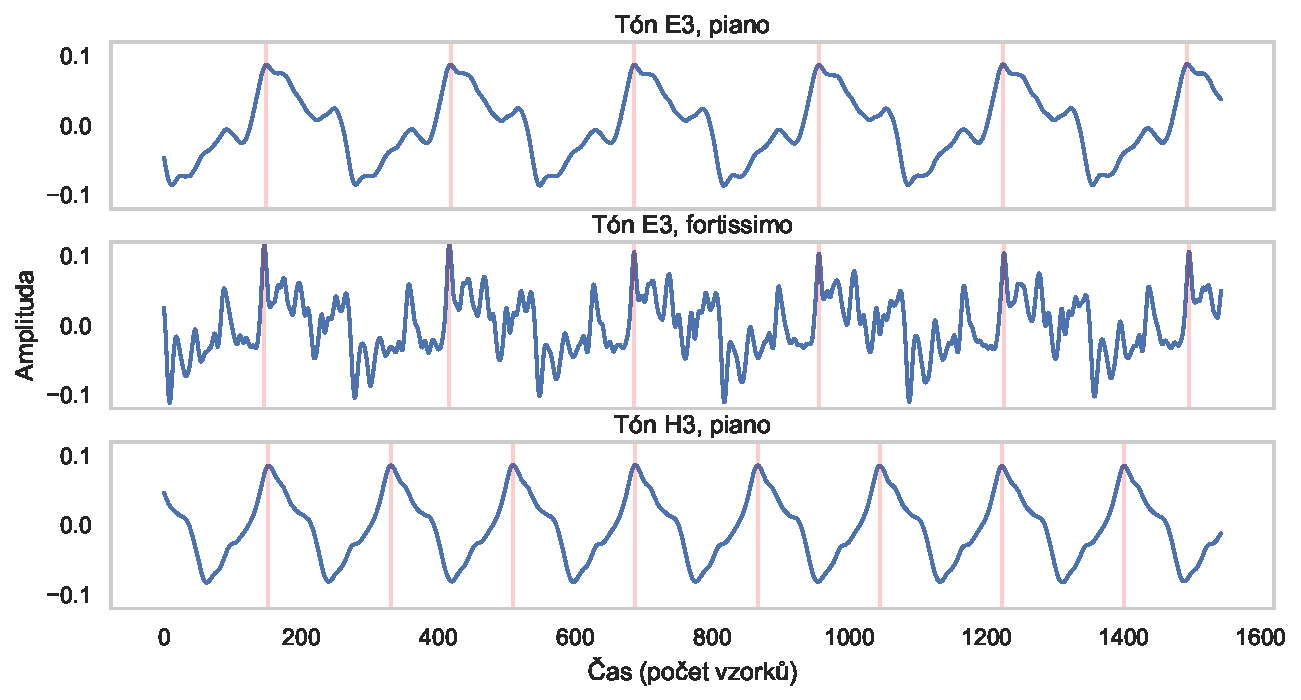
\includegraphics[width=\textwidth,height=\textheight,keepaspectratio]{../img/audio_clarinet}
\caption{Zvuk klarinetu, tóny s různou výškou a dynamikou, 35 milisekund signálu se vzorkovací frekvencí $44\,100\,\rm Hz$. \textcolor{red}{nějak uvést zdroj zvuku \url{https://www.philharmonia.co.uk/explore/sound_samples/clarinet?p=3}}}
\label{obr:audio_clarinet}
\end{figure}

Na obrázku \ref{obr:audio_clarinet} můžeme srovnat tři tóny hrané klarinetem, první dva mají stejnou výšku, jsou ale zahrané s různou intenzitou (dynamikou) \textcolor{red}{je tohle správně formulované, vím že dynamika není intenzita, ale \uv{zahrané s různou dynamikou} mi zní divně?}. Jejich vizuální rozdíl částečně odpovídá i rozdílu v barvě tónu, první tón má příjemný, měkký zvuk; druhý je výraznější a hrubší. Třetí tón se od zbylých liší svou výškou, což lze pozorovat na kratší periodě signálu, která je na obrázku vyznačená úsečkami. 

\begin{figure}[h]\centering
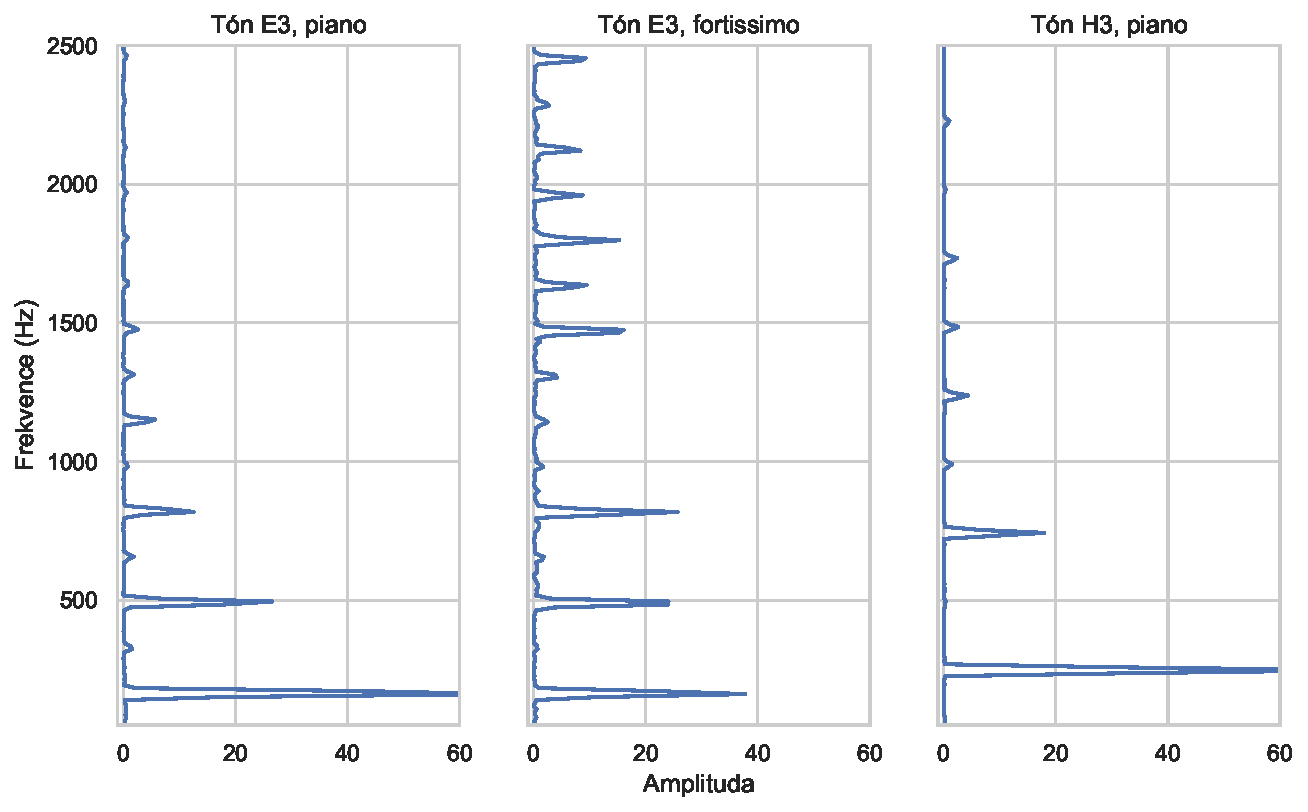
\includegraphics[width=\textwidth,height=\textheight,keepaspectratio]{../img/audio_clarinet_dft}
\caption{Zvuk klarinetu, absolutní hodnota výstupu Fourierovy tranformace signálu délky 4096 s oknem typu Hamming.}
\label{obr:audio_clarinet_dft}
\end{figure}

Jedním ze způsobů analýzy zvukového signálu je pomocí Fourierovy transformace (DFT). Základní myšlenkou je, že na signál lze hledět jako na vážený součet jednodušších signálů. Podobně, jako když se barvy na obrazovce míchají ze tří základních, libovolný zvuk můžeme smíchat ze sady sinusoid. Výslednou kombinaci všech frekvencí, ze kterých se zvuk skládá, označujeme \emph{zvukové spektrum}. Na obrázku \ref{obr:audio_clarinet_dft} vidíme část výsledku Fourierovy transformace zvuků klarinetu z předchozího příkladu. To zásadní, co na spektru tónu můžeme pozorovat, je jeho podstata jakožto součet \emph{harmonických složek}. Tón, kterému posluchač přisoudí výšku $f_0$, se zpravidla skládá ze součtu sinusoid, jejichž frekvence je celočíselným násobkem základní frekvence $f_0$ (jinak také nazývaná \emph{fundamentální frekvence}). Například tedy tón E3 se na obrázku \ref{obr:audio_clarinet_dft} skládá ze složek o frekvenci $165\,\rm Hz$, $330\,\rm Hz$, $495\,\rm Hz$, \dots, zároveň intenzita těchto harmonických frekvencí určuje barvu hlasu.

Ukazuje se, že práce s touto reprezentací zvuku je pro analýzu signálu užitečnější, než práce s nezpracovaným signálem. Ze spektrální reprezentace je například na první pohled zřejmý vztah fundamentálních frekvencí porovnávaných signálů, který odpovídá lidské intuici o výšce zvuků --- tón H3 je na obrázku \ref{obr:audio_clarinet_dft} opravdu \uv{výše} než tón E3. Díky spektrální analýze lze také pozorovat charakteristiky hlasů různých nástrojů. Pro hlas klarinetu platí, že liché harmonické frekvence jsou mnohem výraznější než sudé (na obrázku \ref{obr:audio_clarinet_dft} vypadají sudé harmonické jako malé vrcholky mezi výraznými lichými), naopak například lidský zpěv je charakteristický výraznějšími sudými harmonickými složkami. Další výhodou je možnost hledání rozdílů v barvě tónů --- na spektru vidíme, že vyšší harmonické jsou u tónu hraném fortissimo mnohem výraznější než u tónu hraném piano. Tyto vyšší frekvence způsobují zmiňovanou hrubost tónu. \textcolor{red}{a tohle se dá říct? Tón hraný fortissimo/piano. Moje znalosti hudební terminologie jsou nulové}

Harmonická struktura, která je vlastní lidskému hlasu a téměř všem zvukům hudebních nástrojů, je zásadní pro metody extrakce melodie. Je to vlastnost, která zvuky potenciálně nesoucí melodii odlišuje od bubnového doprovodu, od šumu nebo od jiných nemelodických rušení. Díky ní se také můžeme pokoušet rozložit souzvuk různě vysokých tónů na jejich původní, čisté signály. 

\textcolor{red}{spektrogram hudby - basa, zpěv a bubny. Pod tím obrázek kompletního přepisu melodických kontur}

\begin{figure}[h]\centering
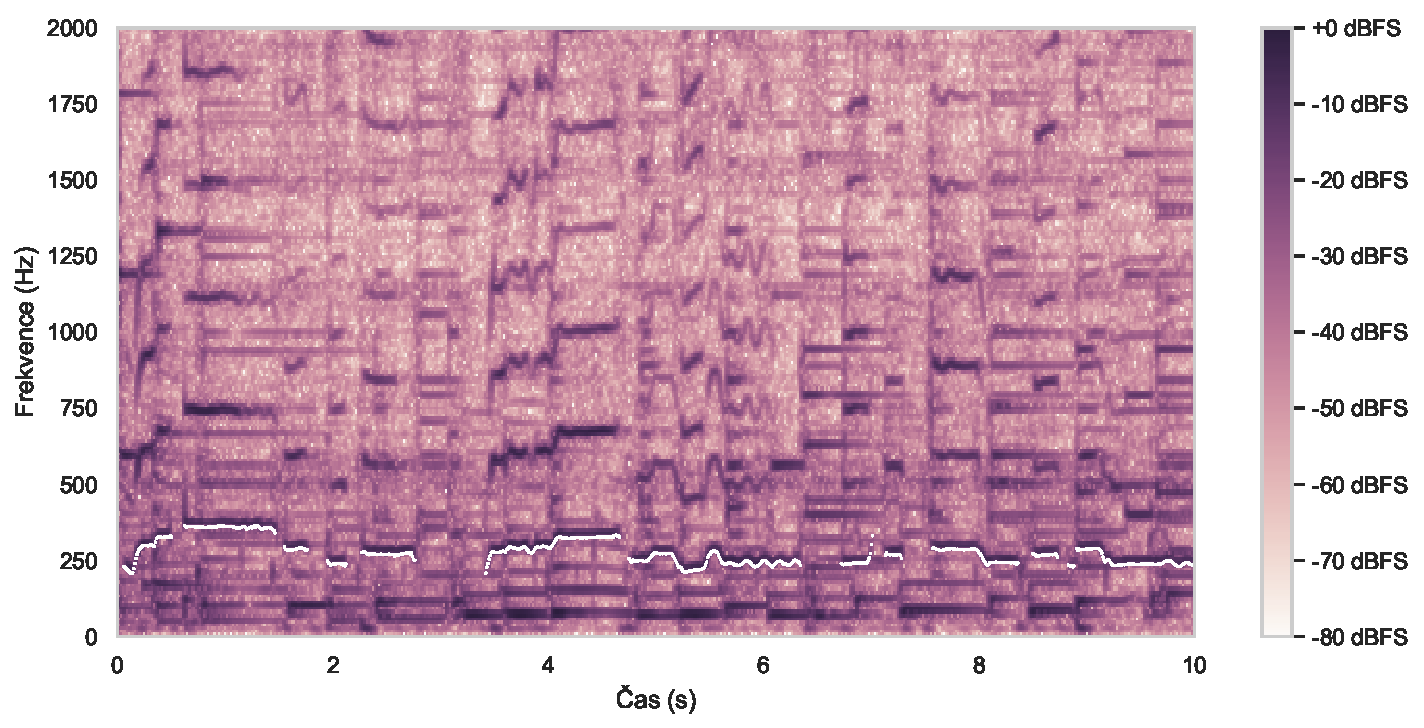
\includegraphics[width=\textwidth,height=\textheight,keepaspectratio]{../img/audio_mix_stft}
\caption{Spektrogram zpěvu s doprovodem piana, basy a perkusí; zpívaná melodie je vyznačena bílým obrysem.}
\label{obr:audio_mix_stft}
\end{figure}

Obrázek \ref{obr:audio_mix_stft} vznikl pomocí opakované Fourierovy transformace, která byla aplikována na po sobě jdoucí, krátké časové úseky vstupní nahrávky, přičemž intenzity frekvenčních složek v každém časovém okamžiku zvuku jsou nyní znázorněny odstínem barvy. Časově-frekvenční reprezentaci signálu nazýváme obecně \emph{spektrogram}, a jeho výpočet je prvním krokem většiny metod pro extrakci melodie.

Na spektrogramu \ref{obr:audio_mix_stft} můžeme pozorovat harmonické struktury tónů --- vyznačenou konturu hlasu, která se na frekvenční ose pohybuje volněji, a pak klavírní a basový doprovod, charakteristický frekvenční stabilitou a v čase slábnoucí amplitudou. Na tomto jednoduchém příkladu lze melodii zpozorovat poměrně snadno, nese ji velmi výrazný, v poměru k doprovodu nejsilnější hlas. Lze na něm však prezentovat první ze základních problémů extrakce melodie.

Frekvence tónů, ze kterých se skládá hudební skladba, jsou uspořádány do stupnic, které definují pevně dané poměry (hudební \emph{intervaly}), ve kterých se tyto tóny ve skladbě mohou vyskytovat. Principem libozvučnosti jsou však takové intervaly, které způsobují, že harmonické frekvence jednotlivých tónů se překrývají a ve výsledné směsi pak není zřejmé, zda-li daná harmonická frekvence patří k jednomu, či více hlasů. Hudební doprovod, pro lidské ucho znějící \uv{pod melodií}, tedy často svými harmonickými frekvencemi zasahuje do melodie samotné, což je zřejmé ze spektrální analýzy.

Dekompozice signálu na jednotlivé znějící hlasy, která je pro člověka přirozená podobně, jako porozumění řeči v rušné kavárně, se kvůli této harmonické povaze tónů a intervalů stává pro algoritmy extrakce melodie obtížným problémem. To, co pro nás činí hudbu zajímavou pro poslech, ji činí obtížně analyzovatelnou pro počítač.


% * další nepříjemnosti
%     * rezonance nástroje po zahrání tónu
%     * dozvuk místnosti
%     * rušení z perkusí
%     * mastering = sice je nahrávka více vyrovnaná, ale problémy přepisu ještě zesiluje
%         * digitální reverb (= dále rozostřuje hranice mezi začátky a konci not, zvětšuje míru překryvů zahraných not)
%         * dynamic range compression = komprese dynamiky zvukového signálu = zmenšuje rozdíly mezi tichými a hlasitými zdroji zvuku
%             * Komprese dynamiky zvukového signálu je proces používaný v audiotechnice ke zmenšení dynamického rozsahu zpracovávaného signálu

\begin{figure}[h]\centering
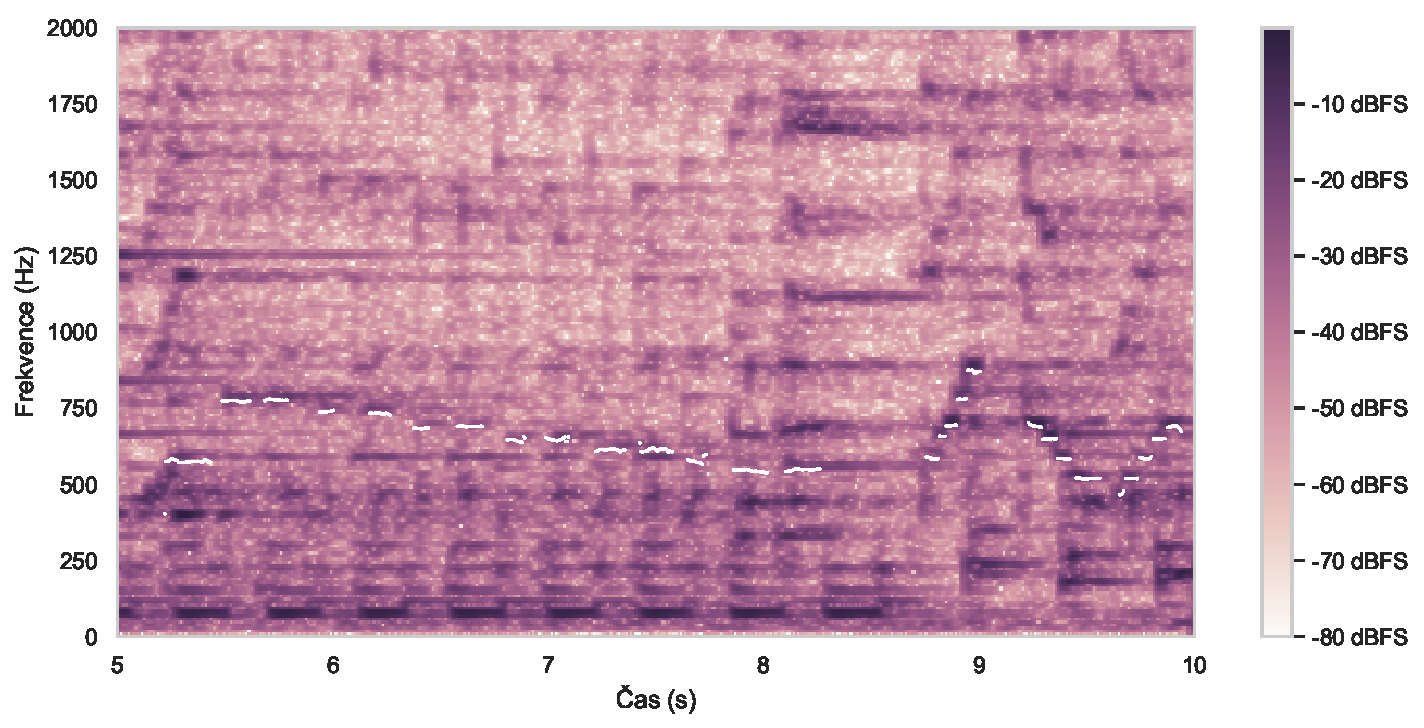
\includegraphics[width=\textwidth,height=\textheight,keepaspectratio]{../img/audio_mix_stft_2}
\caption{Spektrogram orchestrální skladby s obtížně detekovatelnou melodií.}
\label{obr:audio_mix_stft_2}
\end{figure}

\section{Definice melodie}

Rozpoznání melodie v rámci hudební skladby je pro většinu posluchačů intuitivní schopností, která je součástí prožitku poslechu hudby, a která jejímu poslechu vůbec dává smysl. Ačkoli je melodie tedy termín, který je subjektivně jasný, formální, obecně přijímanou muzikologickou definici, která by se zpětně neodkazovala k posluchači, nemá. 

Z tohoto důvodu si výzkumné týmy zabývající se automatickou transkripcí melodie volí pragmaticky spíše užší definice melodie, se kterými se v jejich kontextu pracuje lépe. Práce \cite{Goto1999}, která je považována za jednu z prvních prací v oboru, chápe melodii jako \uv{konturu fundamentální frekvence sestávající se z nejsilnějších tónů hrajících v omezeném frekvenčním rozsahu}. Práce se tedy omezuje na poměrně úzké chápání melodie, obecně se totiž tóny melodie jistě mohou vyskytovat i mimo autory specifikovaný frekvenční rozsah a také nemusí být vždy v poměru s doprovodem nejhlasitější složkou signálu. Z technického hlediska však umožnila autorům implementaci algoritmu běžícího v reálném čase, který poskytoval sémanticky bohatý popis vstupních nahrávek. Navazující články již pracují s volnějšími definicemi, které lépe reflektují podstatu melodie. 

Kompromisem mezi subjektivní a praktickou definicí se na dlouhou dobu stala \uv{extrakce základní frekvence hlavního, neměnného, melodického hlasu}. Ačkoli melodii v reálném hudebním materiálu obvykle nese více hlasů, které se v hraní střídají (například píseň se zpěvem a kytarovým sólem), v letech 2005 -- 2015 se v soutěži MIREX (mezinárodní soutěž pro metody řešící MIR úlohy) provádí evaluace pouze nad krátkými výňatky, kde tato definice není omezující. Přestože se může na první pohled zdát, že tato definice pouze uměle zjednodušuje celou úlohu, její formulace vede k rozvoji nových a zajímavých přístupů, které se sice formálně soustředí právě na extrakci pouze jednoho neměnného hlasu, ale ve výsledku překvapivě dobře fungují i na složitější skladby. Příkladem nového směru může být extrakce melodie pomocí modelování hudebního záznamu jako součtu signálu jednoho hlasu a doprovodu (práce \cite{Durrieu2010} nebo \cite{Bosch2016b}) s přesahem do příbuzné úlohy oddělení hlasů (source separation). Některé práce se zaměřují ještě konkrétněji na separaci lidského zpěvu a doprovodu (\cite{Hsu2010}, \cite{Ikemiya2016}). Nově se také objevují práce, které \uv{hlavní} melodický hlas neinterpretují nutně jako \uv{nejsilnější} a k jeho rozlišení využívají dalších rysů, jako je barva, vibrato nebo délka not. Například \cite{Salamon2012a} využívají těchto rysů pro finální výběr mezi extrahovanými kandidátními konturami.

Ve svém přehledovém článku \cite{Salamon2014} dochází k závěru že výzkum začal v letech 2009--2012 stagnovat, nová data jsou proto pro další vývoj oboru zásadní. Výrazným posunem v rámci MIR komunity proto bylo zveřejnění nových datasetů MedleyDB \citep{Bittner2014} a ORCHSET \citep{Bosch2016}, oba obsahují data, ve kterých již melodii nenese pouze jeden hlas po celou dobu skladby. V porovnání s do té doby dostupnými daty jde také o mnohem rozmanitější kolekce a v případě MedleyDB jde o první volně dostupný dataset, ve kterém se objevují celé skladby, nikoli pouze výňatky.

\cite{Bosch2016} pro práci na datasetu ORCHSET definuje melodii jako \uv{jednohlasou sekvenci tónů, kterou bude posluchač nejspíše reprodukovat, pokud jej požádáme o zapískání či zabroukání příslušné skladby} (na základě článku \cite{Poliner2007}), pro sestavení kolekce dat proto opravdu využívá skupiny posluchačů, které po poslechu krátkých ukázek orchestrální hudby následně žádá o přezpívání melodie. V případě MedleyDB se na anotacích melodie podílí skupina profesionálních hudebníků a vznikají tři různé přepisy melodie s různě volnými formulacemi definice melodie.

Celkový směr výzkumu je tak ve výsledku velmi podmíněn dostupnými daty. Ta tvoří jakýsi protipól k ryze technickým a objektivním cílům algoritmických metod. Nadějí je, že tato dialektika vývoje algoritmů a práce na datech vyústí jednak v metody extrakce, které věrně zachycují podstatu subjektivního prožitku porozumění hudbě, a jednak v celkovém důsledku také snad v lepší porozumění pojmu melodie obecně.

\section{Metody extrakce melodie}

\begin{figure}[h]\centering
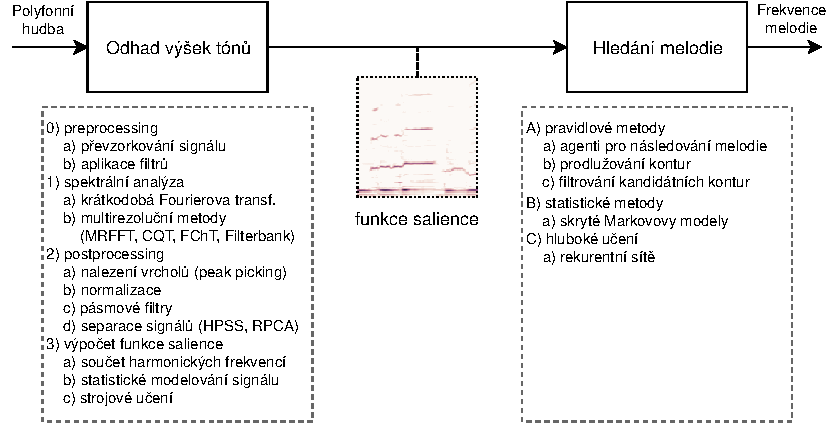
\includegraphics[width=\textwidth,height=\textheight,keepaspectratio]{../img/diagram_systemy_ME}
\caption{Diagram obvyklého návrhu metod pro extrakci melodie.}
\label{obr:diagram_systemy_ME}
\end{figure}

Základním a společným přístupem k problému extrakce melodie je dekompozice na podproblémy odhadu výšek všech znějících hlasů v signálu a následného výběru melodické linie z těchto kandidátních kontur. Jednotlivé metody se pak liší ve způsobech řešení těchto podproblémů, mimo jiné také v míře abstrakce od původního signálu, které při zpracovávání dosahují --- zatímco některé přístupy po celou dobu pracují pouze se signálem jako takovým a důmyslnými způsoby ho transformují tak, aby získaly co nejpřesnější odhad výšky melodie, jiné metody při výpočtu vytváří symbolický popis jednotlivých not a následně i celých frází a melodii pak hledají v tomto vysokoúrovňovém popisu nahrávky. Shrnutí používaných přístupů, blíže popsaných v kapitole \hyperref[chap:souvisejici]{Související práce}, můžeme vidět na diagramu \ref{obr:diagram_systemy_ME}.

\begin{figure}[h]\centering
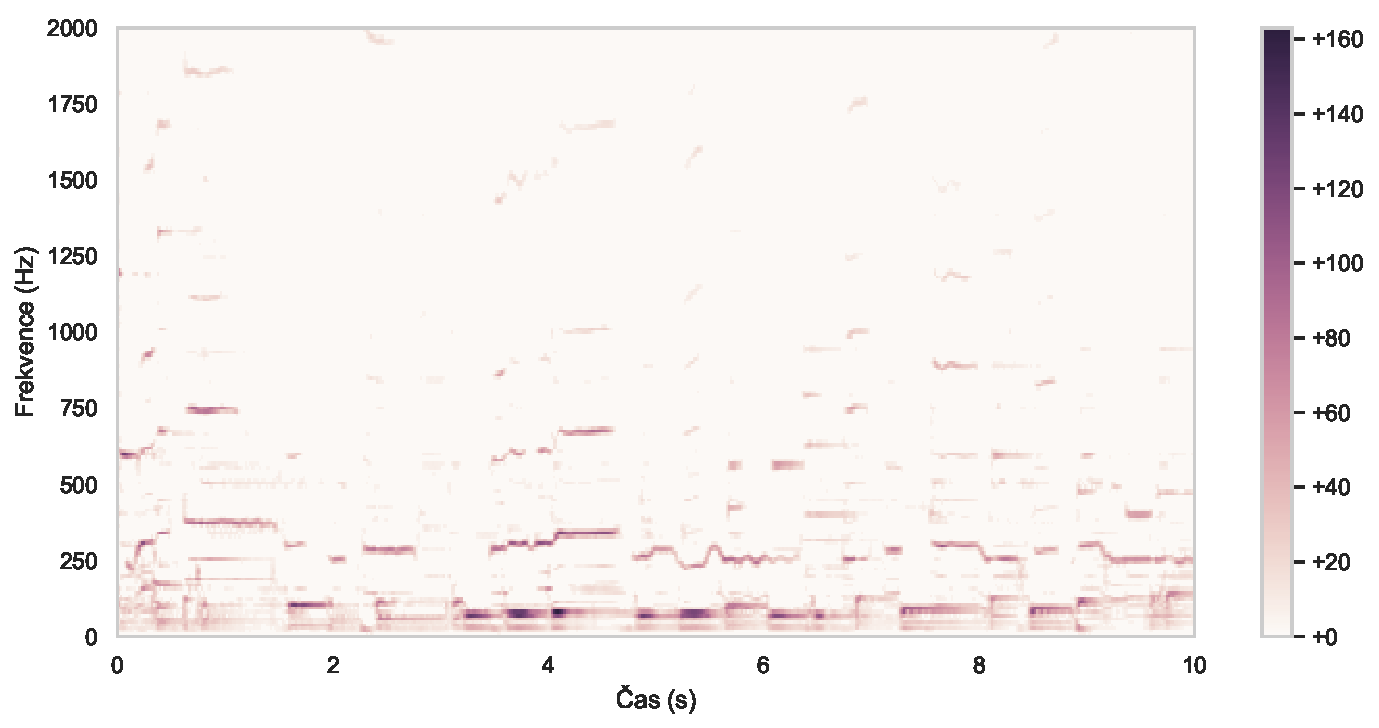
\includegraphics[width=\textwidth,height=\textheight,keepaspectratio]{../img/salience}
\caption{Příklad výstupu výpočtu salienční funkce pomocí váženého sčítání harmonických frekvencí. Ačkoli je zpěv velmi zvýrazněn a salienční funkce na většině nahrávky dobře zachycuje výšku znějící melodie, doprovod kolem čtvrté sekundy nahrávky má vyšší hodnotu než zpěv, což neodpovídá lidskému vnímání zpěvu jakožto nejdůležitější složky signálu.}
\label{obr:salience}
\end{figure}

Prvním krokem všech existujících metod pro extrakci melodie je převod zvukového signálu do frekvenční domény, ať už pomocí zmiňované STFT nebo použitím jiných metod vyvinutých pro analýzu harmonického signálu (MRFFT, CQT, FChT, \dots). Jednou z hlavních výhod těchto dalších metod je logaritmická osa frekvence, díky které je snadné pracovat s harmonickými poměry a hudebními intervaly nezávislé na výšce frekvence. Abychom tuto vlastnost ilustrovali, uvedeme příklad --- tóny A4 a E5 jsou vzdálené o kvintu (na klavíru od tónu A4 musíme postupně zmáčknout 7 bílých a černých klapek, abychom se dostali k tónu E5), tóny A5 a E6 jsou také vzdálené o kvintu. Rozdíl frekvencí těchto tónů je však $220\,\rm Hz$ mezi první dvojicí a $440\,\rm Hz$ mezi druhou dvojicí, tudíž vzdálenost frekvencí daného intervalu závisí na tónu, od kterého se tento interval počítá. Protože je hudební interval jistý \emph{poměr} mezi dvěma tóny, použitím logaritmické osy frekvence se tyto poměry budou jevit jako absolutní rozdíly ($\log n f_0 = \log n + \log f_0$). 

Zpracováním spektrogramu vstupu pak vzniká tzv. \emph{funkce salience}, která každé znějící frekvenci v signálu přiřazuje jisté ohodnocení, které vyjadřuje poměrnou důležitost dané frekvence k ostatním slyšitelným složkám. Funkce salience je tedy v jistém slova smyslu speciální frekvenčně-časová transformace, která podává zejména informace o znějící melodii, nikoli o celkové kompozici signálu. Na obrázku \ref{obr:salience} můžeme srovnat funkci salience vypočtenou pomocí váženého součtu harmonických frekvencí se vstupním spektrogramem \ref{obr:audio_mix_stft}.

Druhým krokem je pak výběr melodie na základě funkce salience. Triviálním řešením je výběr takových frekvencí, které mají nejvyšší ohodnocení. Problémem tohoto přístupu je však to, že jakmile signál obsahuje více podobně ohodnocených tónů, výstup tohoto řešení má tendenci mezi těmito kandidáty často \uv{přeskakovat}. Algoritmy pro extrakci melodie proto volí různě pokročilé metody vyhlazování, případně metody hledání nejpravděpodobnějšího průchodu posloupností stavů (například pomocí Viterbiho algoritmu).

\section{Hluboké učení}

Motivací pro použití metod strojového učení je překonání limitů člověkem navržených, rigidních, pravidlových systémů. Cílem je automatické nalezení optimálního postupu pro řešení úlohy, na základě množství dat, ve kterých strojové učení dokáže nalézt a využít jejich pravidelností. V našem případě pak po metodě založené na strojovém učení požadujeme, aby na základě příkladů z trénovací množiny vytvořila funkci salience.

Výhodou tohoto přístupu je, že o vstupních datech nemusíme dělat žádné předpoklady. Vzniklá metoda pak může v praxi zohledňovat více faktorů ovlivňujících přítomnost melodie, jako je její barva, frekvenční modulace (vibrato, glissando) nebo hlubší vzájemné srovnání současně znějících tónů. Na základě trénovacích příkladů může být tato metoda robustnější vůči většímu spektru barev hlasů nástrojů --- zatímco předešlé metody pro extrakci melodie často uvažují signály s postupně se snižujícím podílem harmonických frekvencí, opravdové signály hudebních nástrojů často tento předpoklad nesplňují (viz obrázek \ref{obr:audio_clarinet_dft}).

První pokus o využití těchto metod představili \cite{Poliner}, vstupní signál transformovali pomocí krátkodobé Fourierovy transformace a část spektra po jednoduché normalizaci použili jako vstupní data pro metodu podpůrných vektorů (SVM). Jejich metoda měla své limitace, výstup byl kvantizován na úroveň jednoho půltónu a tudíž metoda nedokázala dobře postihnout například vibrata. I přesto však tým dosáhl srovnatelných výsledků s ostatními metodami. 

Po roce 2005 jakékoli pokusy o aplikaci strojového učení ustávají a na nové metody se čeká až do roku 2016, jedním z důvodů byl jistě nedostatek dat, tuto situaci zlepšil například dataset MedleyDB \citep{Bittner2014} nebo dnes již zaniklý iKala \citep{Chan2015}. Zájem o strojové učení však znovu stoupá, také díky úspěšnému využití hlubokých neuronových sítí napříč ostatními obory. Na konferenci ISMIR 2016\footnote{International Society for Music Information Retrieval Conference} objevují dva články týmů \cite{Kum2016} a \cite{Rigaud2016}, založené právě na hlubokém učení. V roce 2017 publikuje své metody \cite{Bittner2017} (ISMIR), \cite{Balke2017} (ICASSP\footnote{International Conference on Acoustics, Speech, and Signal Processing}), následující rok přináší metody \cite{DBasaranSEssid2018} (ISMIR), \cite{Bittner2018}. Všechny zmíněné popisujeme v kapitole \hyperref[chap:souvisejici]{Související práce}. V oboru lze tedy od roku 2016 vidět velmi výrazný trend právě směrem k hlubokému učení, a stejný směr je patrný i v příbuzných úlohách přepisu hudby. Tým z laboratoře Google Brain dokázal výrazně zlepšit přepis klavírních skladeb pomocí kombinace konvoluční a rekurentní architektury \citep{Hawthorne2018}. Neuronové sítě také zlepšují výsledky na poli oddělení signálů \citep{Stoller2018}.

V této práci se pokusíme navázat na zmiňované práce a otestovat nové architektury hlubokých neuronových sítí pro úlohu extrakce melodie, zejména pak pro hledání nových způsobů výpočtu funkce salience, v menší míře také pro detekci melodie.

\section{Přínosy práce}

\textcolor{red}{TODO}

\section{Struktura práce}

\textcolor{red}{napsat signpost}

% \cite{Thickstun2016} - musicnet
% \cite{Hawthorne2018} - google magenta

% V oboru transkripce hudby se trend v použití hlubokých sítí